\documentclass[margin=10pt,tikz]{standalone}
%\documentclass[x11names]{article}
\usepackage{tikz}
\usepackage{enumitem}
\usepackage{amsmath}

\usetikzlibrary{shapes,arrows,chains}
%\usepackage{verbatim}
%\usepackage[active,tightpage]{preview}
%\PreviewEnvironment{tikzpicture}
%\setlength\PreviewBorder{5mm}%



\tikzset{
	base/.style={draw, on chain, on grid, align=center, minimum height=4ex},
	proc/.style={base, rectangle, text width=8em},
	ano/.style={base, rectangle, text width=38em, align=left},
	test/.style={base, diamond, aspect=2, text width=5em},
	term/.style={proc, rounded corners},
	% coord node style is used for placing corners of connecting lines
	coord/.style={coordinate, on chain, on grid, node distance=6mm and 25mm},
	% -------------------------------------------------
	% Connector line styles for different parts of the diagram
	norm/.style={->,>=stealth, draw},
}

\begin{document}
%[node distance=2cm]
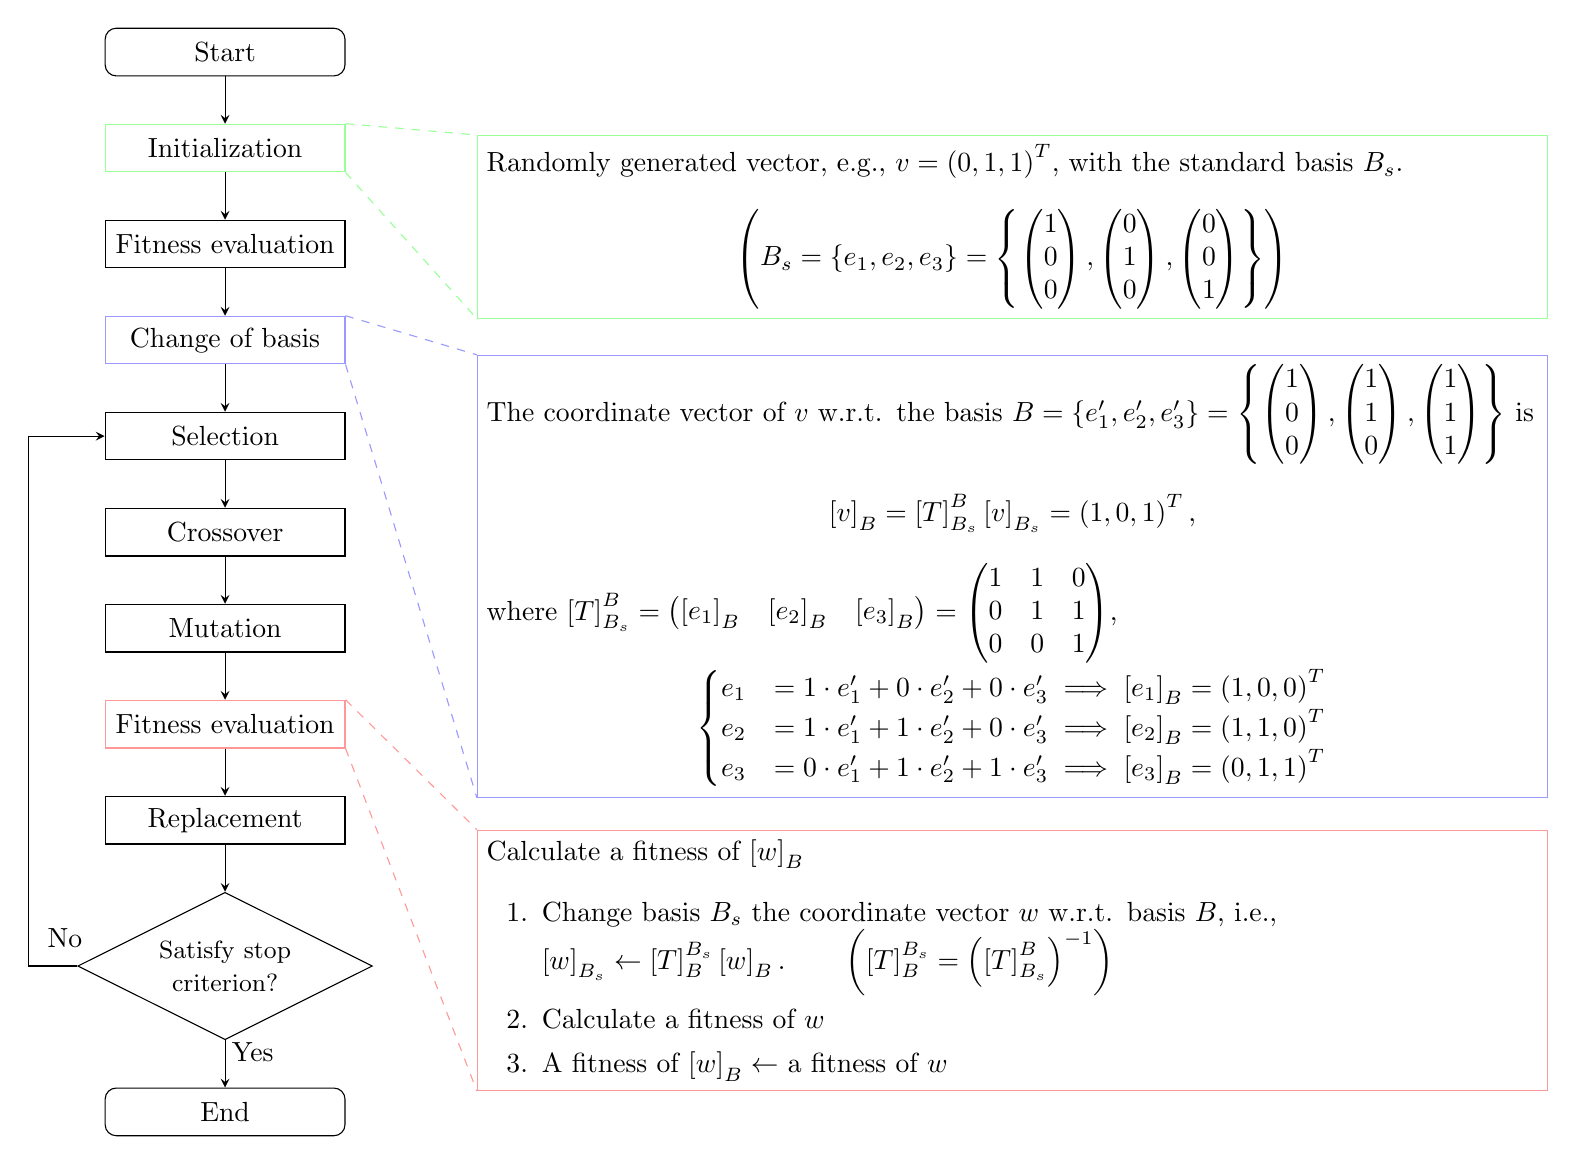
\begin{tikzpicture}[%
	>=triangle 60,              % Nice arrows; your taste may be different
	start chain=going below,    % General flow is top-to-bottom
	node distance=6mm and 60mm, % Global setup of box spacing
	every join/.style={norm},   % Default linetype for connecting boxes
	]
\node [term]       (start)	{Start};
\node [proc, join, draw=green!40] (p1)		{Initialization};
\node [proc, join]			{Fitness evaluation};
\node [proc, join, draw=blue!40] (p2)		{Change of basis};
\node [proc, join] (p3)		{Selection};
\node [proc, join]			{Crossover};
\node [proc, join]			{Mutation};
\node [proc, join, draw=red!40] (p4)		{Fitness evaluation};
\node [proc, join]			{Replacement};
\node [test, join]	(t1)		{\small Satisfy stop criterion?};
\node [term, join]	(ee)		{End};

%
\node [ano, right=of p1, xshift=4cm, yshift=-1cm, draw=green!40] (a1) {Randomly generated vector, e.g., $ v = \left(0, 1, 1\right)^T $, with the standard basis $ B_s $.
\[ \left(B_s = \left\{e_1, e_2, e_3 \right\} = \left\{
\begin{pmatrix} 1 \\ 0 \\ 0\end{pmatrix},
\begin{pmatrix} 0 \\ 1 \\ 0\end{pmatrix},
\begin{pmatrix} 0 \\ 0 \\ 1\end{pmatrix}
\right\}\right) \]};
\node [ano, right=of p2, xshift=4cm, yshift=-3cm, draw=blue!40] (a2) {The coordinate vector of $ v $ w.r.t. the basis $ B = \left\{ e_1^\prime, e_2^\prime, e_3^\prime \right\}
=\left\{ 
	\begin{pmatrix} 1 \\ 0 \\ 0 \end{pmatrix},
	\begin{pmatrix} 1 \\ 1 \\ 0 \end{pmatrix},
	\begin{pmatrix} 1 \\ 1 \\ 1 \end{pmatrix}
\right\} $ is 
\[\left[v \right]_B = \left[T \right]_{B_s}^{B} \left[v \right]_{B_s} = \left(1, 0, 1\right)^T, \]
where $ \left[T \right]_{B_s}^{B} = 
\begin{pmatrix}
\left[e_1\right]_B & \left[e_2\right]_B & \left[e_3\right]_B
\end{pmatrix}
= \begin{pmatrix}
1 & 1 & 0 \\
0 & 1 & 1 \\
0 & 0 & 1
\end{pmatrix} $, \\
\[
\begin{cases}
e_1 &= 1\cdot e_1^\prime + 0 \cdot e_2^\prime + 0 \cdot e_3^\prime \implies \left[e_1\right]_B = \left(1, 0, 0 \right)^T  \\
e_2 &= 1\cdot e_1^\prime + 1 \cdot e_2^\prime + 0 \cdot e_3^\prime \implies \left[e_2\right]_B = \left(1, 1, 0 \right)^T \\
e_3 &= 0\cdot e_1^\prime + 1 \cdot e_2^\prime + 1 \cdot e_3^\prime \implies \left[e_3\right]_B = \left(0, 1, 1 \right)^T
\end{cases}
\]
};
\node [ano, right=of p4, xshift=4cm, yshift=-3cm, draw=red!40] (a4) {Calculate a fitness of $ \left[w\right]_B $\\[0mm]
\begin{enumerate}[leftmargin=7mm, itemsep=0mm]
\item Change basis $ B_s $ the coordinate vector $ w $ w.r.t. basis $ B $, i.e.,\\
$ \left[w\right]_{B_s} \gets \left[T\right]_{B}^{B_s} \left[w\right]_B. \qquad \left(\left[T \right]_B^{B_s} = \left(\left[T \right]_{B_s}^{B}\right)^{-1} \right) $
\item Calculate a fitness of $ w $
\item A fitness of $\left[w\right]_B \gets $ a fitness of $ w $
\end{enumerate}
};

%
\node [coord, left=of t1] (c1)  {};
%
\path (t1.west) to node [near start, yshift=1em] {No} (c1);
  \draw [norm] (t1.west) -- (c1) |- (p3);
\path (t1.south) to node [near start, xshift=1em] {Yes} (ee);

\draw [dashed, draw=green!40] (p1.north east) -- (a1.north west);
\draw [dashed, draw=green!40] (p1.south east) -- (a1.south west);
\draw [dashed, draw=blue!40] (p2.north east) -- (a2.north west);
\draw [dashed, draw=blue!40] (p2.south east) -- (a2.south west);
\draw [dashed, draw=red!40] (p4.north east) -- (a4.north west);
\draw [dashed, draw=red!40] (p4.south east) -- (a4.south west);
\end{tikzpicture}

\end{document}
